\chapter{Introduzione e Analisi di Complessità}

\section{Introduzione}

L'analisi di complessità è il cuore della teoria degli algoritmi. Non basta che un algoritmo sia corretto---deve anche essere \textbf{efficiente}. Ma cosa significa efficienza in senso formale? Come possiamo confrontare due algoritmi che risolvono lo stesso problema? Come possiamo prevedere il comportamento di un algoritmo su input di grandi dimensioni?

Queste domande trovano risposta nell'analisi asintotica, uno strumento matematico che ci permette di caratterizzare il comportamento degli algoritmi al crescere della dimensione dell'input.

\begin{definizione}[Algoritmo]
Un \textbf{algoritmo} è una sequenza finita di istruzioni non ambigue che, dato un input appartenente a un insieme specificato, termina dopo un numero finito di passi producendo un output.
\end{definizione}

Le proprietà fondamentali di un algoritmo sono:
\begin{itemize}
    \item \textbf{Input}: Dati iniziali provenienti da un insieme specificato
    \item \textbf{Output}: Risultato prodotto dall'algoritmo
    \item \textbf{Definitezza}: Ogni passo è definito precisamente
    \item \textbf{Finitezza}: L'algoritmo termina dopo un numero finito di passi
    \item \textbf{Efficacia}: Ogni operazione è sufficientemente basilare da poter essere eseguita
\end{itemize}

\section{Modello di calcolo}

Per analizzare gli algoritmi abbiamo bisogno di un modello di calcolo. Utilizziamo il modello della \textbf{macchina RAM} (Random Access Machine):

\begin{itemize}
    \item Memoria infinita organizzata in celle, ciascuna contenente un numero intero
    \item Accesso a qualsiasi cella in tempo costante $O(1)$
    \item Operazioni aritmetiche di base (+, -, *, /, \%) in tempo costante
    \item Operazioni logiche e di confronto in tempo costante
    \item Un processore che esegue un'istruzione alla volta
\end{itemize}

Questo modello è un'astrazione semplificata ma ragionevole dei computer reali.

\section{Complessità temporale e spaziale}

\begin{definizione}[Complessità temporale]
La \textbf{complessità temporale} di un algoritmo è una funzione $T(n)$ che rappresenta il numero di operazioni elementari eseguite dall'algoritmo su un input di dimensione $n$.
\end{definizione}

\begin{definizione}[Complessità spaziale]
La \textbf{complessità spaziale} di un algoritmo è una funzione $S(n)$ che rappresenta la quantità di memoria utilizzata dall'algoritmo su un input di dimensione $n$.
\end{definizione}

In questo testo ci concentreremo principalmente sulla complessità temporale, anche se entrambe sono importanti nella pratica.

\section{Notazioni asintotiche}

Le notazioni asintotiche ci permettono di descrivere il comportamento di una funzione per valori grandi del suo argomento, ignorando costanti moltiplicative e termini di ordine inferiore.

\subsection{Notazione O-grande (Big-O)}

\begin{definizione}[Notazione O-grande]
Date due funzioni $f(n)$ e $g(n)$ da $\mathbb{N}$ a $\mathbb{R}^+$, diciamo che $f(n) = O(g(n))$ se esistono costanti positive $c$ e $n_0$ tali che:
\[
0 \leq f(n) \leq c \cdot g(n) \quad \forall n \geq n_0
\]
\end{definizione}

In altre parole, $f(n) = O(g(n))$ significa che $f(n)$ cresce al più come $g(n)$ a meno di una costante moltiplicativa, per $n$ sufficientemente grande.

La notazione O-grande fornisce un \textbf{limite superiore asintotico}.

\textbf{Esempi:}
\begin{itemize}
    \item $3n + 5 = O(n)$ perché $3n + 5 \leq 4n$ per $n \geq 5$ (scegliamo $c = 4$, $n_0 = 5$)
    \item $n^2 + 100n + 50 = O(n^2)$ perché $n^2 + 100n + 50 \leq 151n^2$ per $n \geq 1$
    \item $\log n = O(n)$ perché il logaritmo cresce più lentamente di $n$
    \item $2^n = O(3^n)$ ma $3^n \neq O(2^n)$
\end{itemize}

\textbf{Visualizzazione grafica:}

\begin{center}
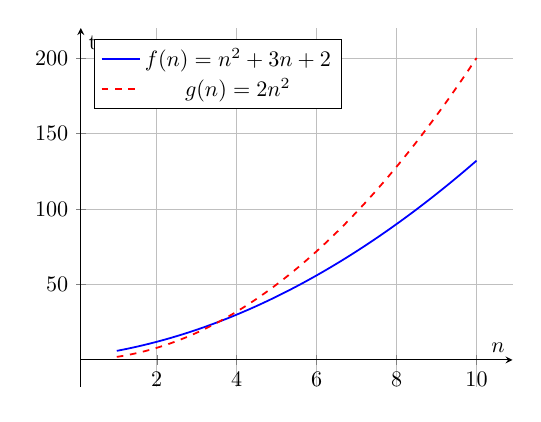
\begin{tikzpicture}[scale=0.8]
    \begin{axis}[
        xlabel={$n$},
        ylabel={tempo},
        domain=1:10,
        samples=100,
        axis lines=middle,
        enlargelimits=true,
        legend pos=north west,
        grid=major
    ]
    \addplot[blue, thick] {x^2 + 3*x + 2};
    \addplot[red, dashed, thick] {2*x^2};
    \legend{$f(n) = n^2 + 3n + 2$, $g(n) = 2n^2$}
    \end{axis}
\end{tikzpicture}
\end{center}

\subsection{Notazione Omega-grande (Big-Omega)}

\begin{definizione}[Notazione Omega-grande]
Date due funzioni $f(n)$ e $g(n)$ da $\mathbb{N}$ a $\mathbb{R}^+$, diciamo che $f(n) = \Omega(g(n))$ se esistono costanti positive $c$ e $n_0$ tali che:
\[
0 \leq c \cdot g(n) \leq f(n) \quad \forall n \geq n_0
\]
\end{definizione}

La notazione Omega-grande fornisce un \textbf{limite inferiore asintotico}.

In altre parole, $f(n) = \Omega(g(n))$ significa che $f(n)$ cresce almeno come $g(n)$ a meno di una costante moltiplicativa.

\textbf{Esempi:}
\begin{itemize}
    \item $5n^2 = \Omega(n^2)$
    \item $n^3 = \Omega(n^2)$ perché $n^3$ cresce più velocemente di $n^2$
    \item $n = \Omega(\log n)$
\end{itemize}

\subsection{Notazione Theta (Big-Theta)}

\begin{definizione}[Notazione Theta]
Date due funzioni $f(n)$ e $g(n)$ da $\mathbb{N}$ a $\mathbb{R}^+$, diciamo che $f(n) = \Theta(g(n))$ se esistono costanti positive $c_1$, $c_2$ e $n_0$ tali che:
\[
0 \leq c_1 \cdot g(n) \leq f(n) \leq c_2 \cdot g(n) \quad \forall n \geq n_0
\]
\end{definizione}

Equivalentemente, $f(n) = \Theta(g(n))$ se e solo se $f(n) = O(g(n))$ e $f(n) = \Omega(g(n))$.

La notazione Theta fornisce un \textbf{limite asintotico stretto}: $f(n)$ e $g(n)$ crescono allo stesso ritmo.

\textbf{Esempi:}
\begin{itemize}
    \item $3n^2 + 5n + 2 = \Theta(n^2)$
    \item $\frac{n^2}{2} - 3n = \Theta(n^2)$
    \item $\log_2 n = \Theta(\log_{10} n)$ (i logaritmi in basi diverse differiscono solo per una costante)
\end{itemize}

\begin{center}
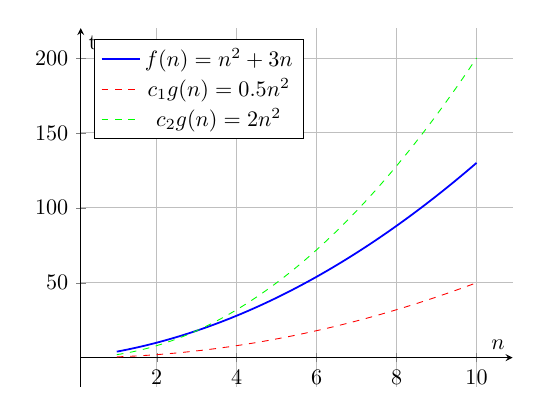
\begin{tikzpicture}[scale=0.8]
    \begin{axis}[
        xlabel={$n$},
        ylabel={tempo},
        domain=1:10,
        samples=100,
        axis lines=middle,
        enlargelimits=true,
        legend pos=north west,
        grid=major
    ]
    \addplot[blue, thick] {x^2 + 3*x};
    \addplot[red, dashed] {0.5*x^2};
    \addplot[green, dashed] {2*x^2};
    \legend{$f(n) = n^2 + 3n$, $c_1 g(n) = 0.5n^2$, $c_2 g(n) = 2n^2$}
    \end{axis}
\end{tikzpicture}
\end{center}

\subsection{Notazioni o-piccolo e omega-piccolo}

Per completezza, introduciamo anche le notazioni asintotiche \textit{strette}:

\begin{definizione}[Notazione o-piccolo]
$f(n) = o(g(n))$ se per ogni costante $c > 0$ esiste $n_0$ tale che:
\[
0 \leq f(n) < c \cdot g(n) \quad \forall n \geq n_0
\]
\end{definizione}

Equivalentemente, $f(n) = o(g(n))$ se:
\[
\lim_{n \to \infty} \frac{f(n)}{g(n)} = 0
\]

\textbf{Esempio:} $n = o(n^2)$ ma $n^2 \neq o(n^2)$

\begin{definizione}[Notazione omega-piccolo]
$f(n) = \omega(g(n))$ se per ogni costante $c > 0$ esiste $n_0$ tale che:
\[
0 \leq c \cdot g(n) < f(n) \quad \forall n \geq n_0
\]
\end{definizione}

\section{Proprietà delle notazioni asintotiche}

\begin{teorema}[Transitività]
Per tutte le funzioni $f, g, h$:
\begin{itemize}
    \item Se $f(n) = O(g(n))$ e $g(n) = O(h(n))$ allora $f(n) = O(h(n))$
    \item Se $f(n) = \Omega(g(n))$ e $g(n) = \Omega(h(n))$ allora $f(n) = \Omega(h(n))$
    \item Se $f(n) = \Theta(g(n))$ e $g(n) = \Theta(h(n))$ allora $f(n) = \Theta(h(n))$
\end{itemize}
\end{teorema}

\begin{proof}
Dimostriamo solo il primo caso (gli altri sono analoghi).

Supponiamo $f(n) = O(g(n))$ e $g(n) = O(h(n))$. Allora esistono costanti $c_1, c_2, n_1, n_2$ tali che:
\begin{align*}
f(n) &\leq c_1 \cdot g(n) \quad \forall n \geq n_1 \\
g(n) &\leq c_2 \cdot h(n) \quad \forall n \geq n_2
\end{align*}

Per $n \geq \max(n_1, n_2)$:
\[
f(n) \leq c_1 \cdot g(n) \leq c_1 \cdot c_2 \cdot h(n)
\]

Ponendo $c = c_1 \cdot c_2$ e $n_0 = \max(n_1, n_2)$, abbiamo $f(n) = O(h(n))$.
\end{proof}

\begin{teorema}[Riflessività]
Per ogni funzione $f(n)$: $f(n) = \Theta(f(n))$
\end{teorema}

\begin{teorema}[Simmetria di Theta]
$f(n) = \Theta(g(n))$ se e solo se $g(n) = \Theta(f(n))$
\end{teorema}

\begin{teorema}[Simmetria trasposta]
$f(n) = O(g(n))$ se e solo se $g(n) = \Omega(f(n))$
\end{teorema}

\section{Classi di complessità comuni}

Ordinate dalla più efficiente alla meno efficiente:

\begin{center}
\begin{tabular}{|l|l|l|}
\hline
\textbf{Notazione} & \textbf{Nome} & \textbf{Esempio} \\
\hline
$O(1)$ & Costante & Accesso a array, operazioni aritmetiche \\
$O(\log n)$ & Logaritmica & Ricerca binaria \\
$O(\sqrt{n})$ & Radice quadrata & Controllo primalità (ingenuo) \\
$O(n)$ & Lineare & Ricerca lineare, scansione array \\
$O(n \log n)$ & Linearitmica & Merge sort, heap sort \\
$O(n^2)$ & Quadratica & Bubble sort, insertion sort \\
$O(n^3)$ & Cubica & Moltiplicazione matrici (ingenua) \\
$O(2^n)$ & Esponenziale & Insieme delle parti, Torre di Hanoi \\
$O(n!)$ & Fattoriale & Permutazioni, problema del commesso viaggiatore (brute force) \\
\hline
\end{tabular}
\end{center}

\textbf{Confronto grafico delle crescite:}

\begin{center}
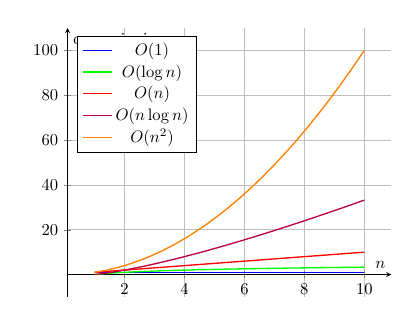
\begin{tikzpicture}[scale=0.6]
    \begin{axis}[
        xlabel={$n$},
        ylabel={operazioni},
        domain=1:10,
        ymax=100,
        axis lines=middle,
        enlargelimits=true,
        legend pos=north west,
        grid=major
    ]
    \addplot[blue, thick] {1};
    \addplot[green, thick] {ln(x)/ln(2)};
    \addplot[red, thick] {x};
    \addplot[purple, thick] {x * ln(x)/ln(2)};
    \addplot[orange, thick] {x^2};
    \legend{$O(1)$, $O(\log n)$, $O(n)$, $O(n \log n)$, $O(n^2)$}
    \end{axis}
\end{tikzpicture}
\end{center}

\section{Tecniche di analisi}

\subsection{Conteggio delle operazioni}

Il metodo più diretto consiste nel contare le operazioni elementari.

\textbf{Esempio: Somma di array}

\begin{lstlisting}[style=pseudocode]
def SommaArray(A, n):
    somma = 0              # 1 operazione
    for i = 1 to n:        # n iterazioni
        somma = somma + A[i]   # 2 operazioni per iterazione
    return somma           # 1 operazione
\end{lstlisting}

Analisi:
\begin{itemize}
    \item Inizializzazione: 1 operazione
    \item Ciclo: $n$ iterazioni $\times$ 2 operazioni = $2n$ operazioni
    \item Return: 1 operazione
    \item Totale: $T(n) = 1 + 2n + 1 = 2n + 2$
\end{itemize}

Quindi: $T(n) = 2n + 2 = \Theta(n)$

\subsection{Cicli annidati}

\textbf{Esempio: Somma di una matrice}

\begin{lstlisting}[style=pseudocode]
def SommaMatrice(M, n):
    somma = 0
    for i = 1 to n:
        for j = 1 to n:
            somma = somma + M[i][j]
    return somma
\end{lstlisting}

Analisi:
\begin{itemize}
    \item Il ciclo esterno esegue $n$ iterazioni
    \item Il ciclo interno esegue $n$ iterazioni per ogni iterazione del ciclo esterno
    \item Operazioni interne: costanti
    \item Totale: $T(n) = c \cdot n \cdot n = cn^2 = \Theta(n^2)$
\end{itemize}

\subsection{Algoritmi ricorsivi}

Per gli algoritmi ricorsivi usiamo le \textbf{relazioni di ricorrenza}.

\textbf{Esempio: Fattoriale}

\begin{lstlisting}[style=pseudocode]
def Fattoriale(n):
    if n == 0:
        return 1
    else:
        return n * Fattoriale(n - 1)
\end{lstlisting}

Relazione di ricorrenza:
\[
T(n) = \begin{cases}
O(1) & \text{se } n = 0 \\
T(n-1) + O(1) & \text{se } n > 0
\end{cases}
\]

Risoluzione:
\begin{align*}
T(n) &= T(n-1) + c \\
     &= T(n-2) + c + c = T(n-2) + 2c \\
     &= T(n-3) + 3c \\
     &\vdots \\
     &= T(0) + nc \\
     &= O(1) + nc = \Theta(n)
\end{align*}

\section{Master Theorem}

Per molti algoritmi ricorsivi di tipo divide-et-impera, il Master Theorem fornisce una soluzione immediata.

\begin{teorema}[Master Theorem - Forma semplificata]
Sia $T(n)$ definita dalla ricorrenza:
\[
T(n) = a \cdot T\left(\frac{n}{b}\right) + f(n)
\]
dove $a \geq 1$, $b > 1$ sono costanti, e $f(n)$ è asintoticamente positiva. Allora:

\begin{enumerate}
    \item Se $f(n) = O(n^{\log_b a - \epsilon})$ per qualche $\epsilon > 0$, allora $T(n) = \Theta(n^{\log_b a})$

    \item Se $f(n) = \Theta(n^{\log_b a})$, allora $T(n) = \Theta(n^{\log_b a} \log n)$

    \item Se $f(n) = \Omega(n^{\log_b a + \epsilon})$ per qualche $\epsilon > 0$, e se $a \cdot f(n/b) \leq c \cdot f(n)$ per qualche $c < 1$ e $n$ sufficientemente grande, allora $T(n) = \Theta(f(n))$
\end{enumerate}
\end{teorema}

\textbf{Esempi di applicazione:}

\textbf{1. Merge Sort:} $T(n) = 2T(n/2) + \Theta(n)$
\begin{itemize}
    \item $a = 2, b = 2, f(n) = \Theta(n)$
    \item $n^{\log_b a} = n^{\log_2 2} = n^1 = n$
    \item $f(n) = \Theta(n) = \Theta(n^{\log_b a})$ → Caso 2
    \item Risultato: $T(n) = \Theta(n \log n)$
\end{itemize}

\textbf{2. Ricerca binaria:} $T(n) = T(n/2) + \Theta(1)$
\begin{itemize}
    \item $a = 1, b = 2, f(n) = \Theta(1)$
    \item $n^{\log_b a} = n^{\log_2 1} = n^0 = 1$
    \item $f(n) = \Theta(1) = \Theta(n^{\log_b a})$ → Caso 2
    \item Risultato: $T(n) = \Theta(\log n)$
\end{itemize}

\textbf{3. Moltiplicazione matrici (Strassen):} $T(n) = 7T(n/2) + \Theta(n^2)$
\begin{itemize}
    \item $a = 7, b = 2, f(n) = \Theta(n^2)$
    \item $n^{\log_b a} = n^{\log_2 7} \approx n^{2.807}$
    \item $f(n) = O(n^{2.807 - \epsilon})$ → Caso 1
    \item Risultato: $T(n) = \Theta(n^{\log_2 7}) \approx \Theta(n^{2.807})$
\end{itemize}

\section{Casi di analisi: Best, Average, Worst}

Un algoritmo può avere comportamenti diversi su input diversi della stessa dimensione. Distinguiamo tre scenari:

\begin{definizione}[Caso migliore (Best Case)]
La complessità nel \textbf{caso migliore} $T_{\text{best}}(n)$ è il tempo minimo richiesto su un input di dimensione $n$.
\end{definizione}

\begin{definizione}[Caso peggiore (Worst Case)]
La complessità nel \textbf{caso peggiore} $T_{\text{worst}}(n)$ è il tempo massimo richiesto su un input di dimensione $n$.
\end{definizione}

\begin{definizione}[Caso medio (Average Case)]
La complessità nel \textbf{caso medio} $T_{\text{avg}}(n)$ è il tempo medio su tutti i possibili input di dimensione $n$, assumendo una distribuzione di probabilità sugli input.
\end{definizione}

\subsection{Esempio: Ricerca lineare}

\begin{lstlisting}[style=pseudocode]
def RicercaLineare(A, n, chiave):
    for i = 1 to n:
        if A[i] == chiave:
            return i
    return -1  // elemento non trovato
\end{lstlisting}

\textbf{Analisi dei casi:}

\begin{itemize}
    \item \textbf{Caso migliore:} La chiave è il primo elemento. $T_{\text{best}}(n) = \Theta(1)$

    \item \textbf{Caso peggiore:} La chiave non è presente o è l'ultimo elemento. $T_{\text{worst}}(n) = \Theta(n)$

    \item \textbf{Caso medio:} Assumendo che la chiave sia presente con uguale probabilità in ogni posizione:
    \[
    T_{\text{avg}}(n) = \frac{1}{n} \sum_{i=1}^{n} i = \frac{1}{n} \cdot \frac{n(n+1)}{2} = \frac{n+1}{2} = \Theta(n)
    \]
\end{itemize}

\subsection{Esempio: Quick Sort}

\textbf{Caso peggiore:} Il pivot è sempre il minimo o il massimo.
\[
T_{\text{worst}}(n) = T(n-1) + T(0) + \Theta(n) = T(n-1) + \Theta(n)
\]

Risoluzione:
\begin{align*}
T(n) &= T(n-1) + cn \\
     &= T(n-2) + c(n-1) + cn \\
     &= T(n-3) + c(n-2) + c(n-1) + cn \\
     &= c \sum_{i=1}^{n} i = c \cdot \frac{n(n+1)}{2} = \Theta(n^2)
\end{align*}

\textbf{Caso migliore:} Il pivot divide sempre a metà.
\[
T_{\text{best}}(n) = 2T(n/2) + \Theta(n) = \Theta(n \log n) \quad \text{(Master Theorem)}
\]

\textbf{Caso medio:} Con un'analisi più complessa si dimostra:
\[
T_{\text{avg}}(n) = \Theta(n \log n)
\]

\section{Limiti inferiori}

Oltre ad analizzare algoritmi specifici, possiamo studiare i \textbf{limiti inferiori} per classi di problemi.

\begin{teorema}[Limite inferiore per l'ordinamento basato su confronti]
Qualsiasi algoritmo di ordinamento basato su confronti richiede $\Omega(n \log n)$ confronti nel caso peggiore per ordinare $n$ elementi.
\end{teorema}

\begin{proof}[Idea della dimostrazione]
Un algoritmo basato su confronti può essere rappresentato come un albero di decisione binario. Ogni foglia corrisponde a una possibile permutazione dell'input. Ci sono $n!$ permutazioni possibili, quindi l'albero deve avere almeno $n!$ foglie.

L'altezza $h$ di un albero binario con $\ell$ foglie soddisfa:
\[
\ell \leq 2^h \implies h \geq \log_2 \ell
\]

Nel nostro caso:
\[
h \geq \log_2(n!) = \sum_{i=1}^{n} \log i \geq \sum_{i=n/2}^{n} \log i \geq \frac{n}{2} \log \frac{n}{2} = \Omega(n \log n)
\]

Quindi qualsiasi algoritmo di ordinamento basato su confronti richiede almeno $\Omega(n \log n)$ confronti.
\end{proof}

Questo teorema implica che algoritmi come Merge Sort e Heap Sort sono \textbf{asintoticamente ottimi} per l'ordinamento basato su confronti.

\section{Complessità spaziale}

Finora ci siamo concentrati sul tempo. Ma la memoria è anch'essa una risorsa importante.

\begin{definizione}[Complessità spaziale]
La \textbf{complessità spaziale} $S(n)$ di un algoritmo è la quantità massima di memoria utilizzata durante l'esecuzione su un input di dimensione $n$.
\end{definizione}

Si distingue tra:
\begin{itemize}
    \item \textbf{Spazio ausiliario}: Memoria extra usata oltre all'input
    \item \textbf{Spazio totale}: Spazio ausiliario + spazio per l'input
\end{itemize}

\textbf{Esempio: Merge Sort}
\begin{itemize}
    \item Spazio ausiliario: $\Theta(n)$ (per l'array temporaneo nella fusione)
    \item Spazio totale: $\Theta(n)$
\end{itemize}

\textbf{Esempio: Quick Sort}
\begin{itemize}
    \item Spazio ausiliario: $\Theta(\log n)$ (per lo stack di ricorsione nel caso medio)
    \item Spazio ausiliario peggiore: $\Theta(n)$ (quando l'albero di ricorsione è sbilanciato)
\end{itemize}

\section{Esercizi}

\subsection{Esercizio 1}
Dimostrare che $2n^2 + 3n + 1 = \Theta(n^2)$.

\subsection{Esercizio 2}
Determinare la complessità asintotica di:
\begin{lstlisting}[style=pseudocode]
def Funzione(n):
    somma = 0
    for i = 1 to n:
        for j = 1 to i:
            somma = somma + 1
    return somma
\end{lstlisting}

\subsection{Esercizio 3}
Risolvere la ricorrenza $T(n) = 3T(n/4) + n^2$ usando il Master Theorem.

\subsection{Esercizio 4}
Analizzare il caso migliore, medio e peggiore della ricerca binaria.

\subsection{Esercizio 5}
Dimostrare che se $f(n) = O(g(n))$ e $g(n) = O(h(n))$, allora $f(n) + g(n) = O(h(n))$.

\section{Conclusioni}

L'analisi di complessità è lo strumento fondamentale per valutare e confrontare algoritmi. Le notazioni asintotiche ci permettono di astrarre dai dettagli implementativi e concentrarci sul comportamento scalabile degli algoritmi.

I concetti chiave di questo capitolo:
\begin{itemize}
    \item Le notazioni O, Omega, Theta caratterizzano limiti superiori, inferiori e stretti
    \item Il Master Theorem risolve molte ricorrenze di tipo divide-et-impera
    \item Gli algoritmi hanno comportamenti diversi nei casi best, average, worst
    \item Esistono limiti inferiori teorici per classi di problemi
    \item La complessità spaziale è importante quanto quella temporale
\end{itemize}

Nei prossimi capitoli applicheremo questi strumenti all'analisi di strutture dati e algoritmi concreti.
